The system results were obtained by evaluating against three recorded sequences from three different kitchens. The sequences were labeled manually using a self-developed labeling program.

\subsection{Evaluation Scores}
In table \ref{tab:evaluation_performance} below the video clips chosen for the evaluation are presented, along with the achieved accuracy measurements. The first 5 minutes of the data set R-Kitchen was used when tuning and developing the system. The data set B25-Kitchen show how robust our system is, since the system wasn't calibrated for the specific room and the camera was slightly miss-placed. The majority of the errors was confirmed to depend on these two factors by ocular inspection.

\begin{table}[h]
\centering
	\begin{tabular}{r | c | c | c | c | c  }
			\emph{Sequence Name}		&  Total entered (GT) & \emph{$A_{in}$} & Total exited (GT) & \emph{$A_{out}$} & length \\
			\hline \hline
			R-Kitchen			& 108 (108) people & 99 \% & 101 (104) people & 97 \% & 32 min\\
			U-Kitchen			& 127 (122) people & 96 \% & 136 (135) people & 99 \% & 31 min  \\
			B25-Kitchen			& 122 (141) people & 87 \% & 77 (91) people & 85 \% & 30 min \\
			\end{tabular}
	\caption[System performance]{\textit{Counting performance according to the evaluation metric as described in section \ref{sec:evaluation}.}}
	\label{tab:evaluation_performance}
\end{table}

Plots of ground truth comparison and accuracy for the evaluation sequences can be found in figure \ref{fig:R-kitchen entries}, \ref{fig:R-kitchen exits}, \ref{fig:B25-kitchen entries} and \ref{fig:B25-kitchen exits}.

\begin{figure}[H]
\centering
\begin{subfigure}{.5\textwidth}
  \centering
  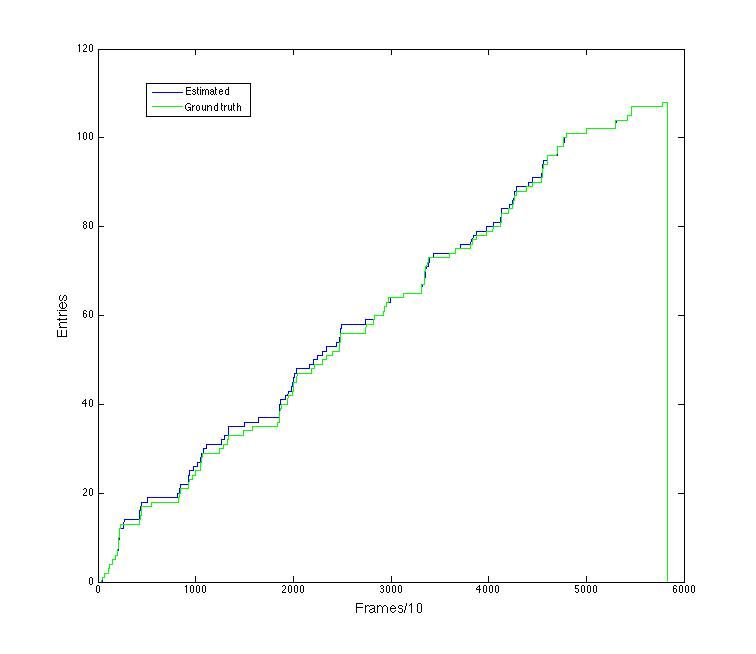
\includegraphics[width=1.1\linewidth]{images/EntriesTest.png}
  \caption{Measured entries and ground truth}
  \label{fig:sub1}
\end{subfigure}%
\begin{subfigure}{.5\textwidth}
  \centering
  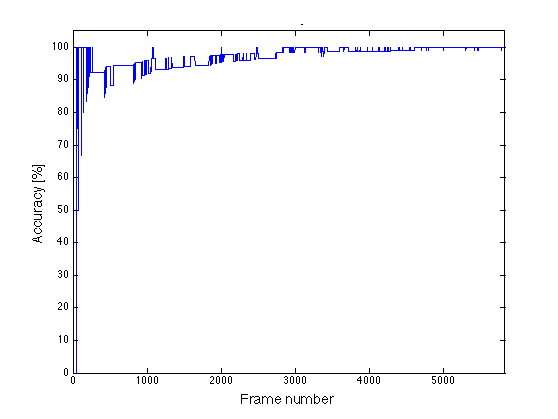
\includegraphics[width=1.1\linewidth]{images/AccEntriesTest.png}
  \caption{Accuracy}
  \label{fig:sub2}
\end{subfigure}
\caption[R-kitchen entries]{\textit{R-Kitchen data. Plot of measured entries, ground truth and accuracy}}
\label{fig:R-kitchen entries}
\end{figure}
\newpage

\begin{figure}[H]
\centering
\begin{subfigure}{.5\textwidth}
  \centering
  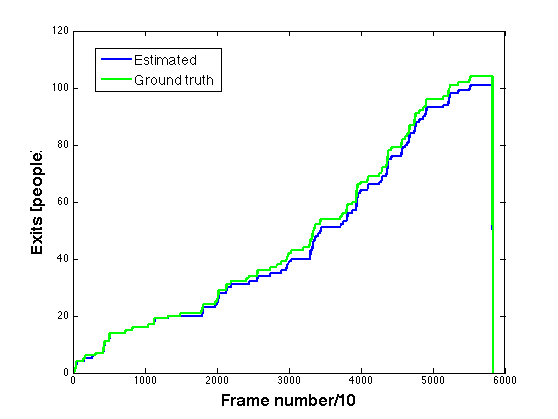
\includegraphics[width=1.1\linewidth]{images/ExitsTest.png}
  \caption{Measured exits and ground truth}
  \label{fig:sub1}
\end{subfigure}%
\begin{subfigure}{.5\textwidth}
  \centering
  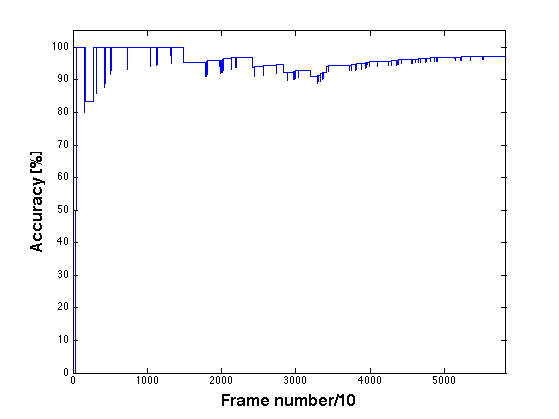
\includegraphics[width=1.1\linewidth]{images/AccExitsTest.png}
  \caption{Accuracy}
  \label{fig:sub2}
\end{subfigure}
\caption[R-kitchen exits]{\textit{R-Kitchen data. Plot of measured exits, ground truth and accuracy}}
\label{fig:R-kitchen exits}
\end{figure}


\begin{figure}[H]
\centering
\begin{subfigure}{.5\textwidth}
  \centering
  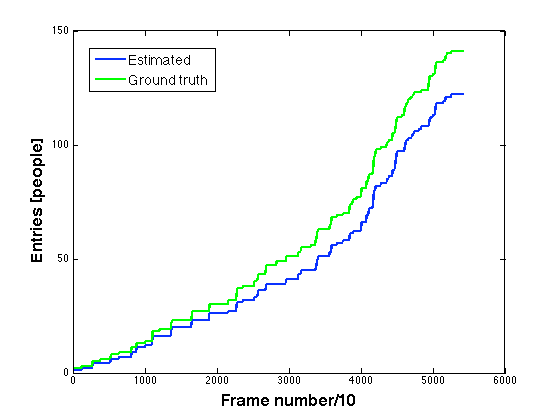
\includegraphics[width=1.1\linewidth]{images/EntriesEval.png}
  \caption{Measured entries and ground truth}
  \label{fig:sub1}
\end{subfigure}%
\begin{subfigure}{.5\textwidth}
  \centering
  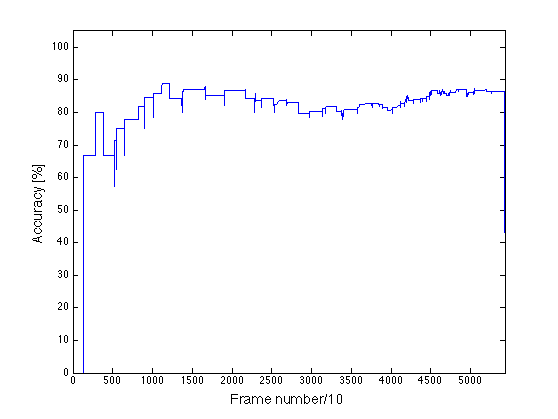
\includegraphics[width=1.1\linewidth]{images/AccEntriesEval.png}
  \caption{Accuracy}
  \label{fig:sub2}
\end{subfigure}
\caption[B25-kitchen entries]{\textit{B25-Kitchen data. Plot of measured entries, ground truth and accuracy}}
\label{fig:B25-kitchen entries}
\end{figure}

\begin{figure}[H]
\centering
\begin{subfigure}{.5\textwidth}
  \centering
  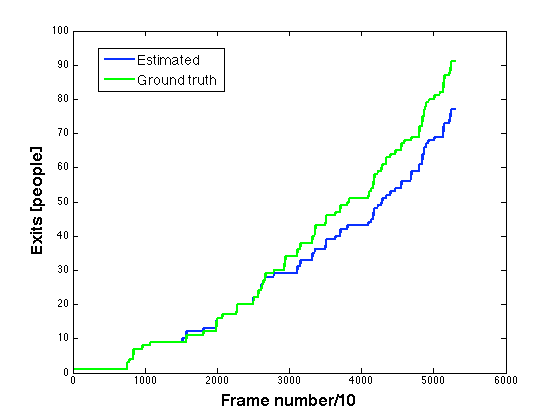
\includegraphics[width=1.1\linewidth]{images/ExitsEval.png}
  \caption{Measured exits and ground truth}
  \label{fig:sub1}
\end{subfigure}%
\begin{subfigure}{.5\textwidth}
  \centering
  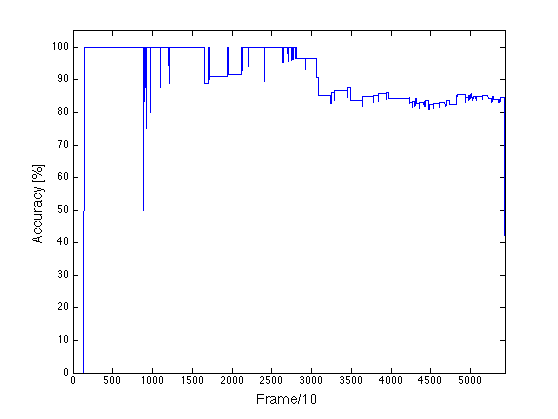
\includegraphics[width=1.1\linewidth]{images/AccExitsEval.png}
  \caption{Accuracy}
  \label{fig:sub2}
\end{subfigure}
\caption[B25-kitchen exits]{\textit{B25-Kitchen data. Plot of measured exits, ground truth and accuracy}}
\label{fig:B25-kitchen exits}
\end{figure}

\subsection{Discussion}
The performance of the R-Kitchen and U-Kitchen sets are very good. The R-Kitchen set is a sequence of 30 minutes, where only the first 5 was used for tuning. The system performed worse on the B25-Kitchen sequence, but that is probably explained by the fact that the sensor was a bit misplaced, making parts of the upper door area on one side to be outside of the field of view, as well as the lack of room-calibration. The reason no more data sets were used was simply that no more time was available.


